
\section{소개}

\begin{itemize}
    \item 일반적으로 가장 많이 사용하는 정렬 알고리즘
    \item 비교 정렬
    \item 내부정렬
    \item 불안정 정렬
    \item 평균 복잡도: $O(n \lg n)$
    \item 최악의 복잡도 : $O(n^2)$
    \item C++ std::sort의 내부구현이 퀵소트로 되어있음\footnote{정확하게는 introsort : quicksort와 heapsort, insertionsort를 셋 다 사용한다.}
\end{itemize}

\section{의사코드 및 동작}

분할 정복(divide and conquer) 방법을 통해 설계 되었다.
작동의 이해는 당장에 유튜브에 검색만해봐도 동작 설명하는 5분짜리 유튜브가 많으니 그걸 참고하는게 편하다.

\begin{lstlisting}[style = CStyle]    
QUICKSORT(A,p,r)
    if p < r
        q = PARTITION(A,p,r)
        QUICKSORT(A,p,q-1)
        QUICKSORT(A,q+1,r)
\end{lstlisting}

\textbf{Lomuto’s Partition Scheme}
\begin{lstlisting}[style = CStyle]
PARTITION(A ,p ,r)
    x= A[r] //pivot
    i = p-1
    for j = p to r-1
        if A[j]<= x
            i = i + 1
            exchange A[i] with A[j]
    exchange A[i+1] with A[r]
    return i + 1
\end{lstlisting}

Hoare, C. A. R.이 1961년 처음으로 Quick sort를 제안했다. PARTITION은 현재 일반적으로 Lomuto가 제안(1999)한 PARTITION이 유명하여 이를 기준으로 설명하며, Hoare가 제안한 Partition의 두 프로시저의 비교는 후에 따로 다룬다.


PARTITION 프로시저의 시간복잡도는 $\Theta(n)$이다.

\begin{figure}[h!]
    \centering
    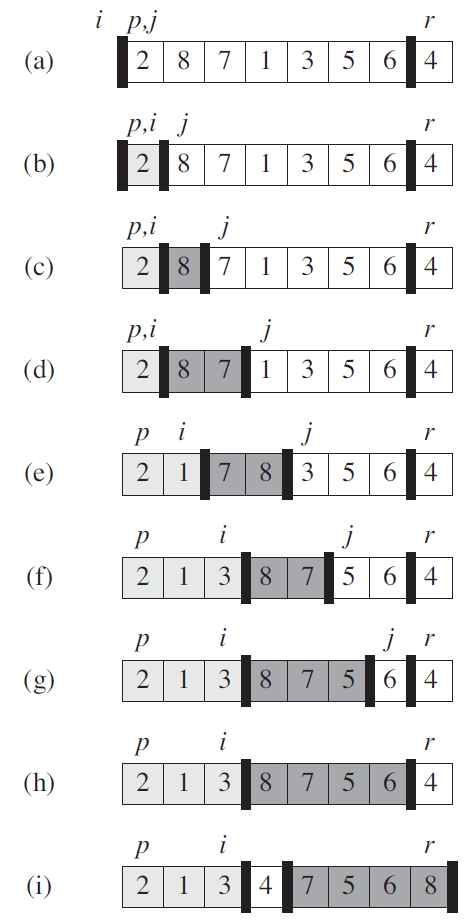
\includegraphics[scale=0.7]{pic/q1.png}
    \caption{quick sort 작동 예시\cite{reference1}}
\end{figure}


%
%성능 참고 : \href{https://www.acmicpc.net/blog/view/58}{정렬 알고리즘 비교}
%정렬 알고리즘 비교
% https://en.wikibooks.org/wiki/LaTeX/Hyperlinks#\hyperref
\newpage
